\chapter{Implementacja algorytmu}

Dane pochodzące ze skanowania laserowego wysokiej rozdzielczości zajmują bardzo dużo miejsca, przez co
dostęp do nich poprzez Internet wymaga relatywnie długiego czasu (rzędu kilkunastu sekund). Powoduje to,
iż niemożliwym jest zbudowanie systemu który w czasie rzeczywistym przedstawiałby te dane w sposób podobny
do aktualnie dostępnych w Internecie map, jak Google Maps. Aby zaradzić temu problemowi, stworzono dwa algorytmy.
Ich celem było takie przetworzenie danych wejsciowych, aby zmiejszyć ich objętość jednoczesnie nie tracąc zawartych w nich informacji.
W niniejszym rozdziale znajdują się opisy tych algorytmów oraz opis przekształcania ich do formatu shapefile w celu udostępnienia
poprzez GeoServer.

\section{Algorytm Naiwny}

W celu szybkiego otrzymania wyników zdecydowano się na stworzenie prostego (naiwnego) algorytmu. Opierał się on na następujących założeniach:
\begin{itemize}
    \item Dane wejściowe posiadają wysoką rozdzielczość (rzędu kilkudziesieciu punktów na metr)
    \item Punkty znajdujące się blisko siebie (tzn. odległość $d$ ze wzoru \ref{eq:odleglosc_euklidesowa} mniejsza niż stała $C$), są fragmentem tej samej powierzchni
\end{itemize}

\noindent Algorytm ten składa się z następujących faz:
\begin{enumerate}
    \item Wczytywanie danych
    \item Wstępne sortowanie
    \item Przypisywanie do zbiorów
    \item Filtracja zbiorów
    \item Znalezienie otoczki wklęsłej dla każdego ze zbiorów
\end{enumerate}

\subsection{Wczytywanie danych}

Dzięki wykorzystaniu biblioteki liblas \cite{website:libLASPython}, odczytywanie danych z plików w formacie .las jest niezwykle proste.
Całość ogranicza się do zaimportowania odpowiedniej klasy i wykorzystania prostej pętli for, jak przedstawiono
w algorytmie \ref{lis:wczytanie_danych}

\begin{lstlisting}[frame=L, language=python, caption={Wczytywanie danych}, label={lis:wczytanie_danych}]
from liblas import file

def read_from_file(name):
    points = []
    f = file.File(name)
    for p in f:
        points.append(MyPoint(p.x, p.y, p.z, classification=p.classification))
    f.close()

    return points
\end{lstlisting}

Punkty są przechowywane w pamięci jako obiekty klasy \textit{MyPoint}. W ramach takiego obiektu przechowywane są informacje dotyczące
współrzędnych punktu, przynależności do zbioru oraz klasyfikacji. Obiekt może też określić swoją odległość od innego punktu
za pomocą metody \textit{get\_distance} oraz określić czy dany punkt jest jego sąsiadem przy użyciu metody \textit{is\_neighbour}.

\subsection{Wstępne sortowanie}
\label{chap:wstepne_sortowanie}

Jak stwierdzono we wstępie, jednym z założeń jest, iż punkty znajdujące się blisko siebie są fragmentem tej samej powierzchni.
Oznacza to konieczność porównywania ze sobą punktów w systemie każdy z każdym, aby stwierdzić, które z nich należą do tego samego zbioru.
Jedakże takie podejście oznacza złożoność obliczeniową rzędu $O(N^2)$, która,  przy ilości punktów wynoszącą kilka milionów, jest niedopuszczalna.
Aby przyspieszyć obliczenia, zdecydowano się na wstępne posortowanie punktów, aby możliwe było porównywanie danego punktu tylko z punktami z 
jego najbliższego otoczenia.

Sortowanie polega na umieszczeniu punktów w macierzy $[M x N]$, której wymiary odpowiadają różnicy między największa i najmniejszą wartością
współrzędnych $x, y$ punktu $p$ ze zbioru punktów wejściowych $P$:
\begin{eqnarray}
    M = max(p.x) - min(p.x) \bigvee p \in P \\
    N = max(p.y) - min(p.y) \bigvee p \in P
\end{eqnarray}

\noindent Punkty umieszczane są w odpowiadjącym ich współrzędnym komórkach macierzy (algorytm \ref{lis:sortowanie_punktow}).

\begin{lstlisting}[frame=L, language=python, caption={Sortowanie punktów}, label={lis:sortowanie_punktow}]
sorted_points = [[ [] for _ in range(0, N)] for _ in range(0, M)]

for p in P:
    x = int(math.floor(p.x - xmin))
    y = int(math.floor(p.y - ymin))
    sorted_points[x][y].append(p)

\end{lstlisting}

W uproszczeniu można powiedzieć, iż algorytm ten powoduje nałożenie siatki na chmurę punktów, co zostało zobrazowane na rysunku \ref{fig:sortowanie_punktow}

\begin{figure}[h!]
	\centering
    \begin{subfigure}[b]{0.3\textwidth}
        \includegraphics[width=\linewidth]{img/sortowanie_punktow1.png}
    \end{subfigure}%
	\quad
    \begin{subfigure}[b]{0.3\textwidth}
        \includegraphics[width=\linewidth]{img/sortowanie_punktow2.png}
    \end{subfigure}%
    \caption{Sortowanie punktów w zbiorze}
    \label{fig:sortowanie_punktow}
\end{figure}

\subsection{Przypisywanie do zbiorów}
W tym etapie następuje podział punktów na podzbiory na podstawie sąsiedztwa. Punkty znajdujące się blisko siebie,
są zaliczane do jednego zbioru i tym samym traktowane jako fragmenty tej samej powierzchni. Dzięki posortowaniu
możliwe jest porównywanie tylko punktów leżących blisko siebie w projekcji dwuwymiarowej (z pominięciem składowej $z$).
Algorytm wygląda następująco:

\begin{lstlisting}[frame=L, language=python, caption={Podział punktów na zbiory w algorytmie naiwnym}, label={lis:podzial_naiwny}]
def find_neighbour(point, neighbour_points, sets):
    if point.point_set is None:
        point.point_set = len(sets)
        sets.append([point])
    for p in neighbour_points:
        if point.is_neighbour(p):
            if p.point_set is None:
                sets[point.point_set].append(p)
                p.point_set = point.point_set
            elif point.point_set != p.point_set:
                union_sets(point.point_set, p.point_set, sets)
\end{lstlisting}

W funkcji przedstawionej na listingu \ref{lis:podzial_naiwny} dokonuje się całe clou algorytmu naiwnego.
W pierwszej części (linie 2-4) aktualnie badany punkt (\textit{point}) tworzy nowy jednoelementowy zbiór,
jeśli nie należy do żadnego.

Następnie punkt ten jest porównywany ze wszystkimi pobliskimi\footnote{pobliskie punkty to takie,
które znajdują się w tej samej lub sąsiedniej komórce macierzy. Patrz \autoref{chap:wstepne_sortowanie}}
punktami. Najpierw sprawdzana jest, czy dwa punkty są sąsiadami tzn. czy leżą na tej samej powierzchni. 
Określa się to poprzez obliczenie odległości $d$ między nimi. Odległość ta jest określana przez metrykę euklidesową:
\begin{equation} \label{eq:odleglosc_euklidesowa_ogolna}
    d(A,B) = \sqrt{\sum\limits_{i=1}^n((x_{iA}-x_{iB})^2)}
\end{equation}

\noindent Gdzie $n$ określa liczbę wymiarów. Dla przypadku trójwymiarowego, równanie \ref{eq:odleglosc_euklidesowa_ogolna} można uprościć do:
\begin{equation} \label{eq:odleglosc_euklidesowa}
    d(A,B) = \sqrt{(x_A - x_B)^2 + (y_A - y_B)^2 + (z_A - z_B)^2}
\end{equation}

Gdzie $x, y, z$ są kolejnymi współrzędymi punktu. Po obliczeniu odległości $d$ na podstawie równania \ref{eq:odleglosc_euklidesowa}
jest sprawdzane, czy jest ona mniejsza niż stała $C$\footnote{Dodatkowo bierze się pod uwagę, czy punkty są tak samo sklasyfikowane.
Jeśli tak, to wtedy $C = C*2$.}. Jeżeli tak, uznaje się że punkty są sąsiadami. Cały proces został zilustrowany na
rysunku \ref{fig:sprawdzanie_sasiedztwa}

\begin{figure}[h!]
    \centering
    \begin{subfigure}[b]{0.3\textwidth}
        \includegraphics[width=\linewidth]{img/sasiedztwo_punktow1.png}
        \caption {punkty należą do tego samego zbioru (d < C)}
    \end{subfigure}
    \quad
    \begin{subfigure}[b]{0.3\textwidth}
        \includegraphics[width=\linewidth]{img/sasiedztwo_punktow2.png}
        \caption {punkty nie należą do tego samego zbioru (d > C)}
    \end{subfigure}%
    \caption{Sprawdzanie sąsiedztwa punktów wobec punktu A}
    \label{fig:sprawdzanie_sasiedztwa}
\end{figure}


Po sprawdzeniu sąsiedztwa, jeżeli drugi z punktów nie należy do żadnego zbioru, przypisuje się go do tego samego zbioru, co badany punkt \textit{point}.
W przeciwnym przypadku (gdy oba punkty należą do różnych zbiorów), zbiory te są łączone przy wykorzystaniu metody \textit{union\_set}.
Metoda ta przepisuje wszystkie punkty z mniejszego zbioru do większego (dbając przy tym o poprawność indeksów).

\subsection{Filtracja zbiorów}

Na tym etapie zostają odrzucone zbiory puste (mogły powstać wskutek łączenia zbiorów) oraz zbiory zawierające
mniej niż $F$ punktów. Pozwala to odrzucić bardzo małe zbiory, które można zaniedbać przy odpowiednim
poziomie szczegółowości.

\subsection{Znalezienie otoczki wklęsłej dla każdego ze zbiorów}

Otoczką wklęsła zbioru punktów na płaszczyźnie nazywamy najmniejszy wielokąt taki, że wszystkie punkty z tego
zbioru leżą albo wewnątrz tego wielokąta, albo na jego krawędziach. Znalezienie tego wielokąta będzie polegało na
stworzeniu najpierw otoczki wypukłej dla zadanego zbioru (przy pomocy triangulacji Delaunaya), a następnie takiego
odfiltrowania krawędzi, aby stworzyć przybliżenie otoczki wklęsłej.

Otoczką wypukłą zbioru punktów na płaszczyźnie nazywamy najmniejszy wielokąt wypukły taki, że wszystkie punkty z tego
zbioru leżą albo wewnątrz tego wielokąta, albo na jego krawędziach \cite{website:OtoczkaTriangulacja}.
Triangulacja Delaunaya jest podziałem otoczki wypukłej na trójkąty. W związku z tym, problem znalezienia otoczki
można sprowadzić do problemu tworzenia triangulacji.

W ramach algorytmu szukamy otoczki zbioru punktów rzutowanych na powierzchnię dwuwymiarową.
Zakładamy, iż każdy znaleziony zbiór jest reprezentacją jakiejś powierzchni płaskiej,
w związku z tym po znalezieniu otoczki, można odrzucić wszystkie punkty znajdujące się wewnątrz.
Będą one interpolowane poprzez punkty graniczne.
Odrzucenie większości punktów skutkuje zmniejszeniem ilości pamięci koniecznej do przechowywania informacji. Jednocześnie autor ma
świadomość ograniczeń tego rozwiązania (wywołanych przez rzutowanie), jak np: upraszczanie ostrosłópów do płaskich powierzchni, co przedstawiono
na rysunku \ref{fig:upraszczanie_otoczki}.

\begin{figure}[h!]
    \centering
    \begin{subfigure}[b]{0.3\textwidth}
        \includegraphics[width=\linewidth]{img/upraszczanie_otoczki1.png}
        \caption {Oryginalne dane}
    \end{subfigure}
    \quad
    \begin{subfigure}[b]{0.3\textwidth}
        \includegraphics[width=\linewidth]{img/upraszczanie_otoczki2.png}
        \caption {Dane po zrzutowaniu}
    \end{subfigure}%
    \caption{Rzutowanie na powierzchnię dwuwymiarową powoduje utracenie części informacji}
    \label{fig:upraszczanie_otoczki}
\end{figure}

Wykorzystanie triangluacji Delaunaya nie jest skomplikowane. Algorytm obliczający triangluacje
dla zbioru punktów jest dostępny jako część pakietu \textit{scipy}. Dodatkowo wykorzystano pakiet \textit{shapely},
który ułatwił zarządzanie figurami geometrycznymi. Cały algorytm (wykorzystujący wspomniane pakiety)
prezentuje się następująco:

\begin{lstlisting}
# Źródło: http://blog.thehumangeo.com/2014/05/12/drawing-boundaries-in-python/
def alpha_shape(points, alpha):
   def add_edge(edges, edge_points, coords, i, j):
        """
        Add a line between the i-th and j-th points,
        if not in the list already
        """
            if (i, j) in edges or (j, i) in edges:
                # already added
                return
            edges.add( (i, j) )
            edge_points.append(coords[ [i, j] ])

    coords = np.array([point.x, point.y
                       for point in points])
    tri = Delaunay(coords)
    edges = set()
    edge_points = []
    # loop over triangles:
    # ia, ib, ic = indices of corner points of the
    # triangle
    for ia, ib, ic in tri.vertices:
        pa = coords[ia]
        pb = coords[ib]
        pc = coords[ic]
        # Lengths of sides of triangle
        a = math.sqrt((pa[0]-pb[0])**2 + (pa[1]-pb[1])**2)
        b = math.sqrt((pb[0]-pc[0])**2 + (pb[1]-pc[1])**2)
        c = math.sqrt((pc[0]-pa[0])**2 + (pc[1]-pa[1])**2)
        # Semiperimeter of triangle
        s = (a + b + c)/2.0
        # Area of triangle by Heron's formula
        area = math.sqrt(s*(s-a)*(s-b)*(s-c))
        circum_r = a*b*c/(4.0*area)
        # Here's the radius filter.
        #print circum_r
        if circum_r < 1.0/alpha:
            add_edge(edges, edge_points, coords, ia, ib)
            add_edge(edges, edge_points, coords, ib, ic)
            add_edge(edges, edge_points, coords, ic, ia)
    m = geometry.MultiLineString(edge_points)
    triangles = list(polygonize(m))
    return cascaded_union(triangles), edge_points 
\end{lstlisting}

Pierwszym etapem tworzenia otoczki wypukłej jest zrzutowanie danych na powierzchnię dwuwymiarową (linie 14-15).
Następnie zostaje utworzona triangulaja Delaunay. Potem następuje przejście po wszystkich trójkątach nowo
utworzonej siatki i dla każdego z nich policzenie promienia okręgu opisanego na tym trójkącie (linie 22-34). Dzięki
parametrowi \textit{alpha} możliwe jest odrzucenie części trójkątów (tych, dla których promień okręgu opisanego jest większy niż $1/alhpa$).
Powoduje to, że otoczka z wypukłej staje się wklęsłą - bardziej odpowiada kształtowi rzeczywistych obiektów.
Ostatnim etapem jest utworzenie obiektu typu \textit{shapely.geometry.polygon.Polygon}. Obiekt ten posiada w sobie informację
o punktach granicznych, tworzących otoczenie. Przykładowe efekty działania funkcji \textit{alpha\_shape} dla różnych wartości 
parametru \textit{alpha} przedstawiono na rysunku \ref{fig:triangulacja_alpha}.

\begin{figure}[h!]
    \centering
    \begin{subfigure}[b]{0.33\textwidth}
        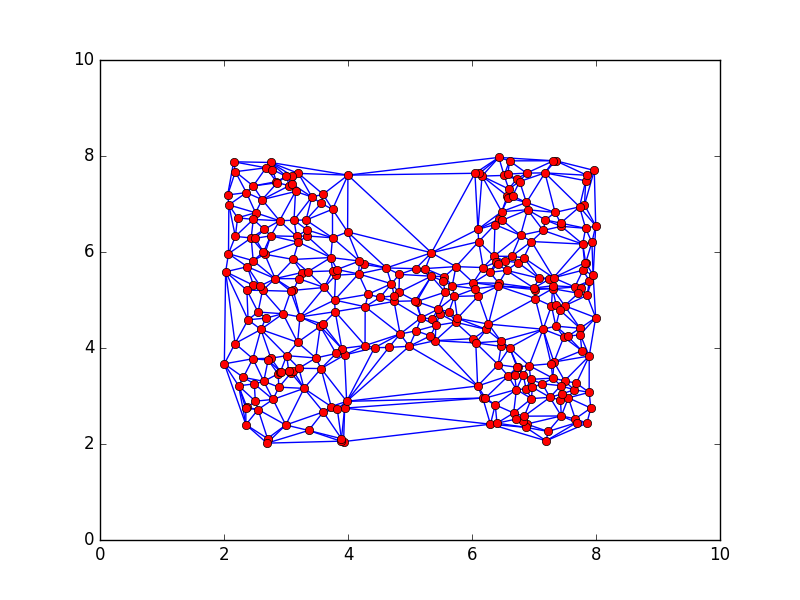
\includegraphics[width=\linewidth]{img/triangulacja1.png}
        \caption {alpha = 0.4}
    \end{subfigure}
    \begin{subfigure}[b]{0.33\textwidth}
        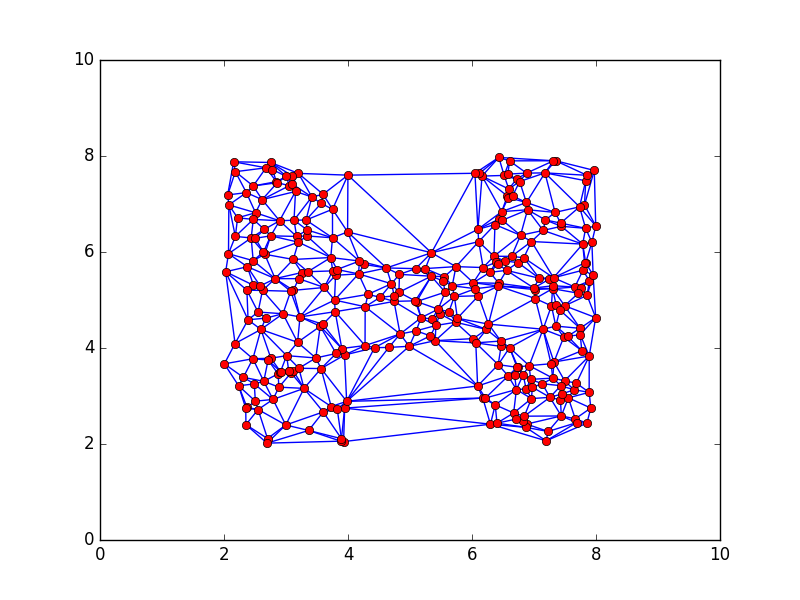
\includegraphics[width=\linewidth]{img/triangulacja2.png}
        \caption {alpha = 0.8}
    \end{subfigure}%
	\begin{subfigure}[b]{0.33\textwidth}
		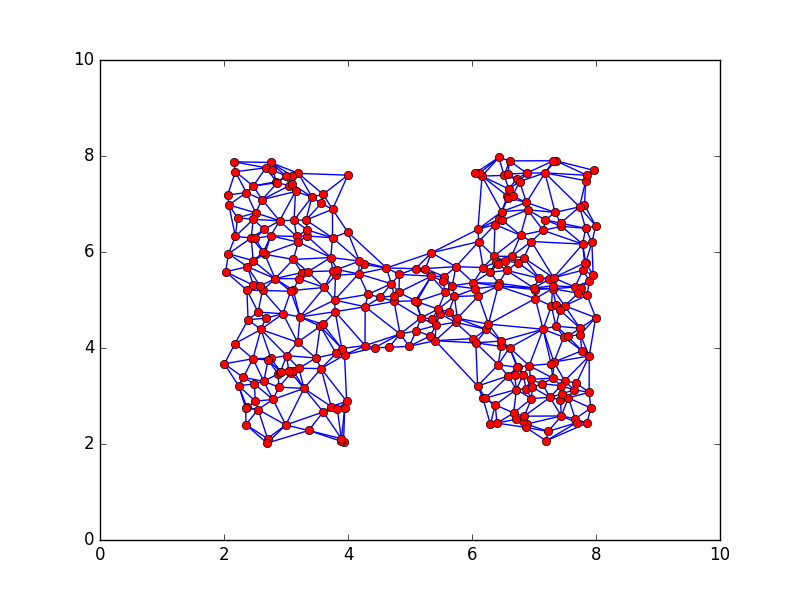
\includegraphics[width=\linewidth]{img/triangulacja3.png}
		\caption {alpha = 1.6}
	\end{subfigure}
    \caption{Efekty metody alpha\_shape przy różnych współczynnikach alpha}
    \label{fig:triangulacja_alpha}
\end{figure}

\section{Algorytm iteracyjny}

Algorytm naiwny dał nadspodziewanie dobre wyniki (\autoref{chap:wyniki}), jednakże posiada jedną wadę:
ciężko poprawić jakość wyników. W związku z tym pojawiła się idea, aby stworzyć nowy algorytm, częściowo
opierając się na poprzednim. W stosunku do algorytmu naiwnego poczyniono następujące zmiany:
\begin{itemize}
    \item Algorytm ma w sposób iteracyjny poprawiać dokładność wyników
    \item Algorytm ma brać pod uwagę też inne czynniki niż odległość punktów od siebie
\end{itemize}

\noindent Kolejne kroki algorytmu pozostały takie same, dla przypomnienia:
\begin{enumerate}
    \item Wczytywanie danych
    \item Wstępne sortowanie
    \item Przypisywanie do zbiorów
    \item Filtracja zbiorów
    \item Znalezienie otoczki wklęsłej dla każdego ze zbiorów
\end{enumerate}

Zmieniony został sposób przypisywania do zbiorów. Na początku wyszukiwane są wszystkie zbiory będące w pobliżu badanego punktu.
Jeżeli nie znaleziono żadnego, tworzy się nowy zbiór zawierający tylko badany punkt.
Jeśli znaleziono jeden zbiór, przypisywano badany punkt do niego.
W syutuacji kiedy znaleziono więcej niż jeden zbiór następuje ważenie. Bierze ono pod uwagę odległość punktu od najbliższego
punktu należącego do zbioru oraz różnicę między średnią wysokością punktów w zbiorze a wysokością badanego punktu podzieloną
przez odchylenie standardowe tego zbioru. Algorytm został przedstawiony na rysunku \ref{fig:algorytm_iteracyjny}. W listingu
\ref{lis:wazenie} przedstawiono jak przebiega faza ważenia.

\begin{figure}[h!]
    \centering
    \includegraphics[width=0.6\linewidth]{img/algorytm_iteracyjny.png}
    \caption{Pętla algorytmu iteracyjnego}
    \label{fig:algorytm_iteracyjny}
\end{figure}

\begin{lstlisting}[frame=L, language=python, label={lis:wazenie}, caption={Ważenie punktów w algorytmie iteracyjnym}]
# calculate which set suits best
max_score = 0
for set_dict in neighbour_sets:
    s = set_dict['set']
    if s.sd() > 0:
        score = abs(s.average() - point.z) / s.sd()
    elif s.sd() == 0.0:
        score = abs(s.average() - point.z) / 0.00001
    set_dict['score'] = score
    if score > max_score:
        max_score = score

max_abs_score = 0
target = None
for set_dict in neighbour_sets:
    if max_score:
        set_dict['score'] = (set_dict['score'] / max_score) / 2.0 + set_dict['distance']
    else:
        set_dict['score'] = set_dict['distance']
    set_dict['score'] = 1 - set_dict['score']

    if set_dict['score'] > max_abs_score:
        target = set_dict
        max_abs_score = set_dict['score']

if point.point_set:
    point.point_set.delete_point(point)
point.point_set = target['set']
target['set'].append(point)
\end{lstlisting}

Fazę ważenia można podzielić na dwa etapy. W pierwszym z nich liczone jest o ile odchyleń standardowych
wartość wysokości danego punktu odbiego od średniej ze zbioru (linie 5-6). Wartość ta stanowi wstępną wartość punktową, jakią uzyskał dany zbiór.
Jeżeli dla danego zbioru odchylenie standardowe wynosi 0\footnote{Będzie tak, jeżeli w zbiorze będzie tylko jeden punkt,
lub gdy wszystkie punkty ze zbioru mają taką samą wysokość.},
wtedy na potrzeby obliczeń przyjmuje się iż odchylenie standardowe jest bardzo małą liczbą ($10^{-5}$).

W drugim etapie następuje normalizacja liczby punktów do przedziału $<0; 0,5>$ poprzez podzielenie wartości punktowej
przez maksymalny wynik uzyskany przez jeden ze zbiorów pomnożonej przez 2. Następnie do znormalizowanego wyniku punktowego
dodaje się odległość\footnote{Odległość jest znormalizowana do przedziału $<0; 0,5>$} 
między badanym punktem a najbliższym punktem ze zbioru (linie 16-17).
Jeżeli maksymlna wartośc punktowa uzyskana w poprzednim etapie wynosi 0, wtedy na potrzeby ostatecznej punktacji
bierze się pod uwagę tylko odległość. Ostateczny wynik uzyskuje się odejmując 1 od uprzednio uzyskanego wyniku (linia 20).
Na końcu przypisuje się punkt do zbioru, który uzyskał największą ilość punktów.

\section{Przekształcanie do formatu shapefile}

Po podziale surowych danych na zbiory (będące w istocie wielokątami), konieczne jest
przekształcenie ich do formatu shapefile. Dzięki temu możliwe będzie wyśwetlanie wyników
za pomocą aplikacji implementujących standardy OGC, jak np: GeoServer.

Do kowersji danych wykorzystano pakiet \textit{osgeo}. Jest to pakiet który umożliwia
wykorzystywanie tzw. bilbioteki GDAL (Geospatial Data Abstraction Library). Pozwala ona
na tworzenie i manipulowanie obiektami geograficznymi, takimi jak punkty, linie i wielokąty.
Dodatkowo posiada wsparcie dla wielu różnych projekcji geograficznych. Wykorzystanie tej
biblioteki do konwersji przedstawiono na listingu \ref{lis:konwersja}.

\begin{lstlisting}[frame=L, language=python, caption={Konwersja danych do formatu SHP}, label={lis:konwersja}]
import osgeo.ogr as ogr
import osgeo.osr as osr

spatialReference = osr.SpatialReference()
spatialReference.ImportFromEPSG(2180)

driver = ogr.GetDriverByName('ESRI Shapefile')
shapeData = driver.CreateDataSource('data.shp')

layer = shapeData.CreateLayer('Layer1', spatialReference, ogr.wkbPolygon)

for surface in surface_list:
	ring = ogr.Geometry(ogr.wkbLinearRing)
	for x, y, z in zip(points[0], points[1], points[2]):
	    ring.AddPoint(x, y, z)
	poly = ogr.Geometry(ogr.wkbPolygon)
	poly.AddGeometry(ring)
	result.append(poly)
	
	feature = ogr.Feature(layer.GetLayerDefn())
	feature.SetGeometry(poly)
	layer.CreateFeature(feature)
	feature.Destroy()

shapeData.Destroy()

\end{lstlisting}

Na początku tworzona jest georeferencja w formacie EPSG 2180 (linie 4-5). Jest to georeferencja w której zostały
zebrane wejściowe dane lidar. Następnie tworzony jest sterownik, w tym wypadku do tworzenia plików .SHP, oraz otwierany
jest deskryptor na plik wynikowy (linie 7-8). Potem tworzona jest nowa warstwa, umieszczana we wcześniej zadeklarowanej
georeferencji. Dodatkowo deklarowane jest, iż warstwa ta zawierać będzie wielokąty (linia 10). W pętli for przechodzimy po kolei
przez wszystkie punkty tworzące wszystkie wielokąty i dodajemy je do stworzonej warstwy (linie 12-23). Na końcu niszczony jest
deskryptor na plik, co powoduje zapisanie przetworzonych informacji na dysku (linia 25).
